%%\documentclass[a4paper,12pt,oneside]{llncs}
\documentclass[12pt,letterpaper]{article}
\usepackage[right=2cm,left=3cm,top=2cm,bottom=2cm,headsep=0cm]{geometry}

%%%%%%%%%%%%%%%%%%%%%%%%%%%%%%%%%%%%%%%%%%%%%%%%%%%%%%%%%%%
%% Juego de caracteres usado en el archivo fuente: UTF-8
\usepackage{ucs}
\usepackage[utf8x]{inputenc}

%%%%%%%%%%%%%%%%%%%%%%%%%%%%%%%%%%%%%%%%%%%%%%%%%%%%%%%%%%%
%% Juego de caracteres usado en la salida dvi
%% Otra posibilidad: \usepackage{t1enc}
\usepackage[T1]{fontenc}

%%%%%%%%%%%%%%%%%%%%%%%%%%%%%%%%%%%%%%%%%%%%%%%%%%%%%%%%%%%
%% Ajusta maergenes para a4
%\usepackage{a4wide}

%%%%%%%%%%%%%%%%%%%%%%%%%%%%%%%%%%%%%%%%%%%%%%%%%%%%%%%%%%%
%% Uso fuente postscript times, para que los ps y pdf queden y pequeños...
\usepackage{times}

%%%%%%%%%%%%%%%%%%%%%%%%%%%%%%%%%%%%%%%%%%%%%%%%%%%%%%%%%%%
%% Posibilidad de hipertexto (especialmente en pdf)
%\usepackage{hyperref}
\usepackage[bookmarks = true, colorlinks=true, linkcolor = black, citecolor = black, menucolor = black, urlcolor = black]{hyperref}

%%%%%%%%%%%%%%%%%%%%%%%%%%%%%%%%%%%%%%%%%%%%%%%%%%%%%%%%%%%
%% Graficos 
\usepackage{graphics,graphicx}

%%%%%%%%%%%%%%%%%%%%%%%%%%%%%%%%%%%%%%%%%%%%%%%%%%%%%%%%%%%
%% Ciertos caracteres "raros"...
\usepackage{latexsym}

%%%%%%%%%%%%%%%%%%%%%%%%%%%%%%%%%%%%%%%%%%%%%%%%%%%%%%%%%%%
%% Matematicas aun más fuertes (american math dociety)
\usepackage{amsmath}

%%%%%%%%%%%%%%%%%%%%%%%%%%%%%%%%%%%%%%%%%%%%%%%%%%%%%%%%%%%
\usepackage{multirow} % para las tablas
\usepackage[spanish,es-tabla]{babel}

%%%%%%%%%%%%%%%%%%%%%%%%%%%%%%%%%%%%%%%%%%%%%%%%%%%%%%%%%%%
%% Fuentes matematicas lo mas compatibles posibles con postscript (times)
%% (Esto no funciona para todos los simbolos pero reduce mucho el tamaño del
%% pdf si hay muchas matamaticas....
\usepackage{mathptm}

%%% VARIOS:
\usepackage{slashbox}
\usepackage{verbatim}
\usepackage{array}
\usepackage{listings}
\usepackage{multirow}

%% MARCA DE AGUA
%% Este package de "draft copy" NO funciona con pdflatex
%%\usepackage{draftcopy}
%% Este package de "draft copy" SI funciona con pdflatex
%%%\usepackage{pdfdraftcopy}
%%%%%%%%%%%%%%%%%%%%%%%%%%%%%%%%%%%%%%%%%%%%%%%%%%%%%%%%%%%
%% Indenteacion en español...
\usepackage[spanish]{babel}

\usepackage{listings}
% Para escribir código en C
% \begin{lstlisting}[language=C]
% #include <stdio.h>
% int main(int argc, char* argv[]) {
% puts("Hola mundo!");
% }
% \end{lstlisting}


\title{Análisis}
\author{Jesús Rodríguez Heras}

\begin{document}
	
	\maketitle
	\begin{abstract} %Poner esto en todas las prácticas de PCTR
		\begin{center}
			Análisis de resultados del ejercicio 1 de la práctica 12.
		\end{center}
	\end{abstract}
	\thispagestyle{empty}
	\newpage
	
%	\tableofcontents
%	\newpage
	
	%%\listoftables
	%%\newpage
	
	%%\listoffigures
	%%\newpage
	
	%%%% REAL WORK BEGINS HERE:
	
	%%Configuracion del paquete listings
	\lstset{language=bash, numbers=left, numberstyle=\tiny, numbersep=10pt, firstnumber=1, stepnumber=1, basicstyle=\small\ttfamily, tabsize=1, extendedchars=true, inputencoding=latin1}

\section{Tiempos para el ejercicio 1}
\subsection{Windows}
\begin{center}
	\begin{table}[htbp]
		\begin{center}
			\begin{tabular}{|c|c|c|c|c|}
				\hline
				& \multicolumn{2}{c|}{C++} & \multicolumn{2}{c|}{Java}  \\
				\hline
				Intentos  & piSecuencial & piParalelo & piSecuencial & piParalelo \\\hline
				100000 & 0.247 & 0.032 & 0.016 & 0.032 \\\hline
				1000000 & 2.408 & 0.231 & 0.1 & 0.122 \\\hline
				10000000 & 24.038 & 2.143 & 0.63 & 0.955 \\\hline
				20000000 & 48.122 & 15.894 & 1.263 & 1.919 \\\hline
			\end{tabular}
			\caption{Valores en segundos del tiempo usado por cada algoritmo.}
			\label{tabla:Valores en segundos del tiempo usado por cada algoritmo}
		\end{center}
	\end{table}
\end{center}


\subsection{Linux}
\begin{center}
	\begin{table}[htbp]
		\begin{center}
			\begin{tabular}{|c|c|c|c|c|}
				\hline
				& \multicolumn{2}{c|}{C++} & \multicolumn{2}{c|}{Java}  \\
				\hline
				Intentos  & piSecuencial & piParalelo & piSecuencial & piParalelo \\\hline
				100000 & 0.026 & 0.019 & 0.016 & 0.027 \\\hline
				1000000 & 0.223 & 0.109 & 0.072 & 0.123 \\\hline
				10000000 & 2.127 & 0.943 & 0.593 & 1.124 \\\hline
				20000000 & 4.248 & 1.884 & 1.205 & 2.241 \\\hline
			\end{tabular}
			\caption{Valores en segundos del tiempo empleado por cada algoritmo.}
			\label{tabla:Valores en segundos del tiempo empleado por cada algoritmo}
		\end{center}
	\end{table}
\end{center}
\section{Gráficas}
\newpage

\begin{center}
	\begin{figure}
		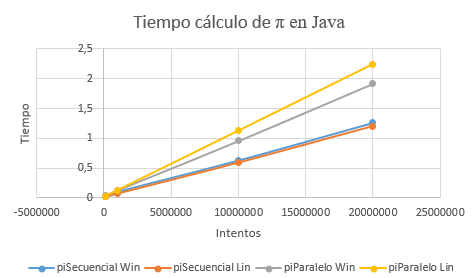
\includegraphics[scale=1.3]{TiempoPiJava.png}
	\end{figure}
\end{center}

\begin{center}
	\begin{figure}
		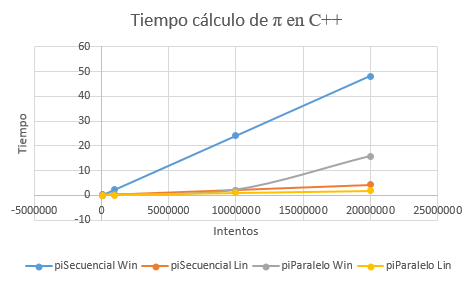
\includegraphics[scale=1.3]{TiempoPiC.png}
	\end{figure}
\end{center}

\begin{center}
	\begin{figure}
		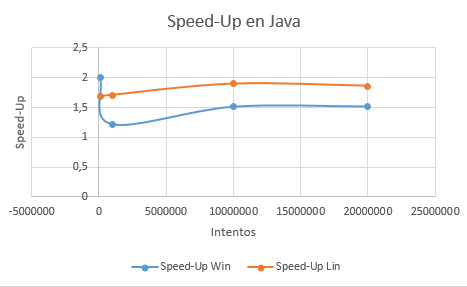
\includegraphics[scale=1.3]{SpeedUpJava.png}
	\end{figure}
\end{center}

\begin{center}
	\begin{figure}
		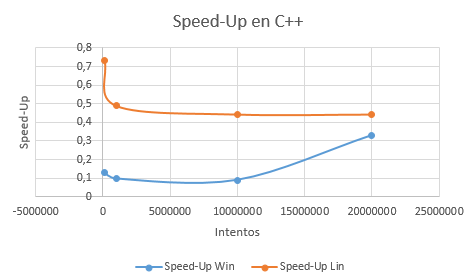
\includegraphics[scale=1.3]{SpeedUpC.png}
	\end{figure}
\end{center}




%\begin{table}[]
%	\centering
%	
%	\begin{tabular}{|c|c|c|c|c|c|c|c|c|}\hline
%		& \multicolumn{4}{c}{C++}                                           & \multicolumn{4}{c}{Java}                                          \\\hline
%		Vueltas  & Secuencial W10 & Secuencial Linux & Paralelo W10 & Paralelo Linux & Secuencial W10 & Secuencial Linux & Paralelo W10 & Paralelo Linux \\\hline
%		100000   & 0.247          & 0.026            & 0.032        & 0.019          & 0.016          & 0.016            & 0.032        & 0.027          \\\hline
%		1000000  & 2.408          & 0.223            & 0.231        & 0.109          & 0.1            & 0.072            & 0.122        & 0.123          \\\hline
%		10000000 & 24.038         & 2.127            & 2.143        & 0.943          & 0.63           & 0.593            & 0.955        & 1.124          \\\hline
%		20000000 & 48.122         & 4.248            & 15.984       & 0.1884         & 1.263          & 1.205            & 1.919        & 2.241\\\hline
%	\end{tabular}
%\caption{My caption}
%\label{my-label}
%\end{table}



\end{document}